\tikzset{%
    every neuron/.style={
        circle,
        draw,
        minimum size=5pt,
        inner sep=0pt,
        very thin
    },
    neuron/.style={
        fill
    },
}
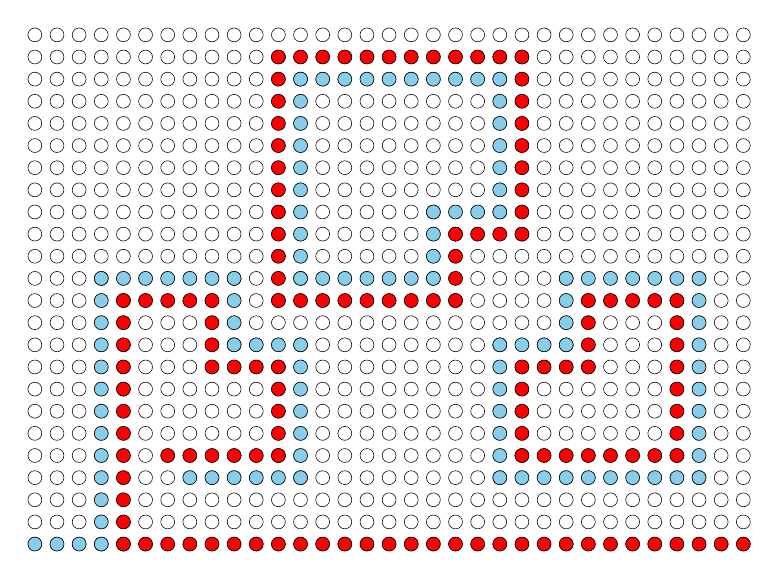
\begin{tikzpicture}[x=0.8cm, y=0.8cm, >=latex, every text node part/.style={align=center}]
    \foreach \x in {0,...,32}
        \foreach \y in {0,...,23} {
            % \pgfmathtruncatemacro{\label}{\x - 5 *  \y +21}
            \node [every neuron/.try] (\x,\y) at (8pt*\x,8pt*\y) {};
        } 
    \foreach \x in {0,...,3}
        \foreach \y in {0,...,0} {
            % \pgfmathtruncatemacro{\label}{\x - 5 *  \y +21}
            \node [every neuron/.try, fill=SkyBlue] (\x,\y) at (8pt*\x,8pt*\y) {};
        } 
    \foreach \x in {4,...,32}
        \foreach \y in {0,...,0} {
            % \pgfmathtruncatemacro{\label}{\x - 5 *  \y +21}
            \node [every neuron/.try, fill=Red] (\x,\y) at (8pt*\x,8pt*\y) {};
        } 
    \foreach \x in {3,...,3}
        \foreach \y in {0,...,12} {
            % \pgfmathtruncatemacro{\label}{\x - 5 *  \y +21}
            \node [every neuron/.try, fill=SkyBlue] (\x,\y) at (8pt*\x,8pt*\y) {};
        } 
    \foreach \x in {4,...,4}
        \foreach \y in {0,...,11} {
            % \pgfmathtruncatemacro{\label}{\x - 5 *  \y +21}
            \node [every neuron/.try, fill=Red] (\x,\y) at (8pt*\x,8pt*\y) {};
        } 
    \foreach \x in {3,...,9}
        \foreach \y in {12,...,12} {
            % \pgfmathtruncatemacro{\label}{\x - 5 *  \y +21}
            \node [every neuron/.try, fill=SkyBlue] (\x,\y) at (8pt*\x,8pt*\y) {};
        } 
    \foreach \x in {4,...,8}
        \foreach \y in {11,...,11} {
            % \pgfmathtruncatemacro{\label}{\x - 5 *  \y +21}
            \node [every neuron/.try, fill=Red] (\x,\y) at (8pt*\x,8pt*\y) {};
        } 
    \foreach \x in {9,...,9}
        \foreach \y in {9,...,12} {
            % \pgfmathtruncatemacro{\label}{\x - 5 *  \y +21}
            \node [every neuron/.try, fill=SkyBlue] (\x,\y) at (8pt*\x,8pt*\y) {};
        } 
    \foreach \x in {8,...,8}
        \foreach \y in {9,...,11} {
            % \pgfmathtruncatemacro{\label}{\x - 5 *  \y +21}
            \node [every neuron/.try, fill=Red] (\x,\y) at (8pt*\x,8pt*\y) {};
        } 
    \foreach \x in {9,...,12}
        \foreach \y in {9,...,9} {
            % \pgfmathtruncatemacro{\label}{\x - 5 *  \y +21}
            \node [every neuron/.try, fill=SkyBlue] (\x,\y) at (8pt*\x,8pt*\y) {};
        } 
    \foreach \x in {8,...,11}
        \foreach \y in {8,...,8} {
            % \pgfmathtruncatemacro{\label}{\x - 5 *  \y +21}
            \node [every neuron/.try, fill=Red] (\x,\y) at (8pt*\x,8pt*\y) {};
        } 
    \foreach \x in {12,...,12}
        \foreach \y in {3,...,9} {
            % \pgfmathtruncatemacro{\label}{\x - 5 *  \y +21}
            \node [every neuron/.try, fill=SkyBlue] (\x,\y) at (8pt*\x,8pt*\y) {};
        } 
    \foreach \x in {11,...,11}
        \foreach \y in {4,...,8} {
            % \pgfmathtruncatemacro{\label}{\x - 5 *  \y +21}
            \node [every neuron/.try, fill=Red] (\x,\y) at (8pt*\x,8pt*\y) {};
        } 
    \foreach \x in {7,...,12}
        \foreach \y in {3,...,3} {
            % \pgfmathtruncatemacro{\label}{\x - 5 *  \y +21}
            \node [every neuron/.try, fill=SkyBlue] (\x,\y) at (8pt*\x,8pt*\y) {};
        } 
    \foreach \x in {6,...,11}
        \foreach \y in {4,...,4} {
            % \pgfmathtruncatemacro{\label}{\x - 5 *  \y +21}
            \node [every neuron/.try, fill=Red] (\x,\y) at (8pt*\x,8pt*\y) {};
        } 
    \foreach \x in {12,...,12}
        \foreach \y in {12,...,21} {
            \node [every neuron/.try, fill=SkyBlue] (\x,\y) at (8pt*\x,8pt*\y) {};
        }
    \foreach \x in {12,...,21}
        \foreach \y in {21,...,21} {
            \node [every neuron/.try, fill=SkyBlue] (\x,\y) at (8pt*\x,8pt*\y) {};
        }
    \foreach \x in {21,...,21}
        \foreach \y in {15,...,21} {
            \node [every neuron/.try, fill=SkyBlue] (\x,\y) at (8pt*\x,8pt*\y) {};
        }
    \foreach \x in {18,...,18}
        \foreach \y in {12,...,15} {
            \node [every neuron/.try, fill=SkyBlue] (\x,\y) at (8pt*\x,8pt*\y) {};
        }
    \foreach \x in {12,...,18}
        \foreach \y in {12,...,12} {
            \node [every neuron/.try, fill=SkyBlue] (\x,\y) at (8pt*\x,8pt*\y) {};
        }
    \foreach \x in {18,...,21}
        \foreach \y in {15,...,15} {
            \node [every neuron/.try, fill=SkyBlue] (\x,\y) at (8pt*\x,8pt*\y) {};
        }
    
    \foreach \x in {11,...,11}
        \foreach \y in {11,...,22} {
            \node [every neuron/.try, fill=Red] (\x,\y) at (8pt*\x,8pt*\y) {};
        }
    \foreach \x in {11,...,22}
        \foreach \y in {22,...,22} {
            \node [every neuron/.try, fill=Red] (\x,\y) at (8pt*\x,8pt*\y) {};
        }
    \foreach \x in {22,...,22}
        \foreach \y in {14,...,22} {
            \node [every neuron/.try, fill=Red] (\x,\y) at (8pt*\x,8pt*\y) {};
        }
    \foreach \x in {19,...,19}
        \foreach \y in {11,...,14} {
            \node [every neuron/.try, fill=Red] (\x,\y) at (8pt*\x,8pt*\y) {};
        }
    \foreach \x in {11,...,19}
        \foreach \y in {11,...,11} {
            \node [every neuron/.try, fill=Red] (\x,\y) at (8pt*\x,8pt*\y) {};
        }
    \foreach \x in {19,...,22}
        \foreach \y in {14,...,14} {
            \node [every neuron/.try, fill=Red] (\x,\y) at (8pt*\x,8pt*\y) {};
        }

    \foreach \x in {30,...,30}
        \foreach \y in {12,...,3} {
            \node [every neuron/.try, fill=SkyBlue] (\x,\y) at (8pt*\x,8pt*\y) {};
        }
    \foreach \x in {30,...,21}
        \foreach \y in {3,...,3} {
            \node [every neuron/.try, fill=SkyBlue] (\x,\y) at (8pt*\x,8pt*\y) {};
        }
    \foreach \x in {21,...,21}
        \foreach \y in {9,...,3} {
            \node [every neuron/.try, fill=SkyBlue] (\x,\y) at (8pt*\x,8pt*\y) {};
        }
    \foreach \x in {24,...,24}
        \foreach \y in {12,...,9} {
            \node [every neuron/.try, fill=SkyBlue] (\x,\y) at (8pt*\x,8pt*\y) {};
        }
    \foreach \x in {30,...,24}
        \foreach \y in {12,...,12} {
            \node [every neuron/.try, fill=SkyBlue] (\x,\y) at (8pt*\x,8pt*\y) {};
        }
    \foreach \x in {24,...,21}
        \foreach \y in {9,...,9} {
            \node [every neuron/.try, fill=SkyBlue] (\x,\y) at (8pt*\x,8pt*\y) {};
        }

    \foreach \x in {29,...,29}
        \foreach \y in {11,...,4} {
            \node [every neuron/.try, fill=Red] (\x,\y) at (8pt*\x,8pt*\y) {};
        }
    \foreach \x in {29,...,22}
        \foreach \y in {4,...,4} {
            \node [every neuron/.try, fill=Red] (\x,\y) at (8pt*\x,8pt*\y) {};
        }
    \foreach \x in {22,...,22}
        \foreach \y in {8,...,4} {
            \node [every neuron/.try, fill=Red] (\x,\y) at (8pt*\x,8pt*\y) {};
        }
    \foreach \x in {25,...,25}
        \foreach \y in {11,...,8} {
            \node [every neuron/.try, fill=Red] (\x,\y) at (8pt*\x,8pt*\y) {};
        }
    \foreach \x in {29,...,25}
        \foreach \y in {11,...,11} {
            \node [every neuron/.try, fill=Red] (\x,\y) at (8pt*\x,8pt*\y) {};
        }
    \foreach \x in {25,...,22}
        \foreach \y in {8,...,8} {
            \node [every neuron/.try, fill=Red] (\x,\y) at (8pt*\x,8pt*\y) {};
        }
\end{tikzpicture}